\documentclass[11pt]{article}
\pdfpxdimen=1in
\divide\pdfpxdimen by 300
 
\usepackage[latin1]{inputenc}
\usepackage[english]{babel}
\usepackage{mathtools, bm}
\usepackage{amssymb, bm}
\usepackage{float}

\usepackage{caption} % to center captions
\usepackage{subcaption} % subcaption for figures side by side

\usepackage{booktabs} % for super cool table
\usepackage[table,xcdraw]{xcolor}  % to put color in tables
\usepackage{tcolorbox} % add box
\usepackage{commath} % for absolute values

\usepackage[parfill]{parskip}
\usepackage{graphicx}
\usepackage{hyperref}
\usepackage[top=0.8in, bottom=0.8in, left=1in, right=1in]{geometry}
\usepackage{listings}
\usepackage{framed}

\usepackage{array}

\newcommand*{\horzbar}{\rule[.5ex]{2.5ex}{0.5pt}} % for horizontal line in matrix

\renewcommand\thesubsection{\thesection.\arabic{subsection}} % Subsection starting with A, B, ...

\renewcommand\thefigure{\thesubsection.\arabic{figure}}

\newcommand{\horrule}[1]{\rule{\linewidth}{#1}} % Create horizontal rule command with 1 argument of height

\numberwithin{figure}{section} % to have per-section figure numbering

\title{	
\normalfont \normalsize 
\textsc{Master MVA \\
Convex Optimization} \\ [20pt]
\horrule{0.5pt} \\[0.2cm] % Thin top horizontal rule
\textbf{Homework 3}: Algorithms Implementation \\
\horrule{2pt} \\[0.3cm] % Thick bottom horizontal rule
}

\author{Victor Busa \\
   \texttt{victor.busa@ens-paris-saclay.fr}}

\date{\normalsize\today}

\begin{document}

\maketitle

\section{Interior Points Method}

\paragraph{Compute $\nabla_{\phi_t(x)}$ and $\nabla^2_{\phi_t(x)}$}

Let's define $\phi_t(x)$ by:

$$
\phi_t(x) = t\left(\frac{1}{2}x^{\intercal}Qx + p^{\intercal}x\right) + \mathcal{B}(b - Ax)
$$

then if we note $A = \left[
  \begin{array}{ccc}
    \horzbar & a^{T}_{1} & \horzbar \\
    \horzbar & a^{T}_{2} & \horzbar \\
             & \vdots    &          \\
    \horzbar & a^{T}_{m} & \horzbar
  \end{array}
\right], \in \mathbb{R}^{m \times n}$, we can compute $\nabla_{\phi_t(x)}$ as follow:

\begin{align*}
\nabla_{\phi_t(x)} &= t(p + Qx) - \sum\limits_{i=1}^m \frac{-a_i}{b_i - a^{\intercal}_i x} \\
&= t(p + Qx) + \sum\limits_{i=1}^m a_i \frac{1}{b_i - a^{\intercal}_i x} \\
&= t(p + Qx) + A^{\intercal}d
\end{align*}

Where we defined $d$, the vector in $\mathbb{R}^{m}$, s.t $d = \begin{pmatrix} 
1/(b_1 - a^{\intercal}_1 x) \\
\vdots \\
1/(b_m - a^{\intercal}_m x) 
\end{pmatrix}$

Then, we can compute the Hessian of $\phi_t(x)$, as follow:

\begin{align*}
\nabla^2_{\phi_t(x)} &= tQ + \sum\limits_{i=1}^m \frac{a_i a^{\intercal}_i}{(b_i - a^{\intercal}_i x)^2} \\
&= tQ + A^{\intercal} diag(d)^2 A
\end{align*}

Where we've reused the vector $d$ defined earlier.

\paragraph{implementation of phi, grad and hess} See Python code

\section{Newton Method}
\paragraph{implementation of dampedNewtonStep} See Python code
\paragraph{implementation of dampedNewton} See Python code
\paragraph{implementation of newtonLS} See Python code

\section{Support Vector Machine Problem}
\paragraph{3.1 Strictly feasible points for primal and dual}
\subparagraph{a) For the dual:} the dual problem is:

\begin{equation}\tag*{(SVM-D)}
	\begin{split}
	\text{maximize} \quad & \mathbf{1}^{\intercal} \lambda - \frac{1}{2} \norm{\sum\limits_{i=1}^n \lambda_i y_i x_i}^{2}_2 \\
	\text{subject to} \quad & 0 \leq \lambda \leq \frac{1}{\tau n}
	\end{split}
\end{equation}

So, as we are maximizing over $\lambda$ only, we can take $\lambda$ that satisfies $0 < \lambda < 1/(\tau n)$, to have a strictly feasible
point. For example one can use $\lambda = 1/(2 \tau n)$ as a strictly feasible point for (SVM-D).

\subparagraph{b) For the primal:} the primal problem is:

\begin{equation}\tag*{(SVM-P)}
	\begin{split}
	\text{minimize} \quad & \frac{1}{\tau n} \sum\limits_{i=1}^n z_i + \frac{1}{2} \norm{w}^{2}_2 \\
	\text{subject to} \quad & y_i(w^{\intercal} x_i) \geq 1 - z_i, \quad i=1, \hdots, n \\
	& z \geq 0
	\end{split}
\end{equation}

Here, we are maximizing over both $w$ and $z$. We can see that if we define $Y = diag(y_1, \hdots, y_n)$, then:
$(Xw)_i = \sum\limits_{k=1}^d X_{ik}w_k = x^{\intercal}_i w = w^{\intercal} x_i$, so $y_i(w^{\intercal} x_i) =(YXw)_i$.
And the strictly feasible points are such that $\forall i \in [1,n]$, $z_i + y_i(w^{\intercal} x_i) > 1$ and $z > 0$, so
in particular, strictly feasible points must satisfy:

\begin{align*}
z + YXw > \mathbf{1} \\
z > 0
\end{align*}

So, for example, one can use $z = c \times \mathbf{1}$ and $w = \mathbf{0}_{d}$ where $c$ is a constant with $c > 1$ as a strictly feasible point for (SVM-P).

\paragraph{3.2 Barrier method implementation}
\subparagraph{a) Transform (SVM-D) and (SVM-P) as (QP)}
Let's define $X = (x_1, \hdots, x_n) \in \mathbb{R}^{d \times n}$, $y \in \{-1, 1\}^{n}$ and $\tau > 0$. Let's first transform the primal problem
into a QP. \\

In the primal problem, we have $x = \begin{pmatrix} 
w \\
z 
\end{pmatrix}$

and we want:

$$
\frac{1}{2}x^{\intercal} Q x = \frac{1}{2}\norm{w}^{2}_2
$$

by identification it comes:

\begin{framed} 
$$
Q = \begin{pmatrix} 
I_{d,d} &  0_{d,n}\\
0_{n,d} & 0_{n,n}
\end{pmatrix}
$$
\end{framed} 

Where the subscripts represent the sizes of the bloc matrices. \\

In the same way, we want:

$$
p^{\intercal} x = p^{\intercal}\begin{pmatrix} 
w \\
z 
\end{pmatrix} =  \frac{1}{\tau n} \mathbf{1}^{\intercal} z
$$

And by identification, we have naturally:

\begin{framed} 
$$
p = \frac{1}{\tau n} \begin{pmatrix} 
0_{d} \\
1_{n}
\end{pmatrix}
$$
\end{framed} 

Finally, the constraint $Ax \leq b$ can be rewritten:

$$
\begin{pmatrix} 
A_{{11}_{n,d}} & A_{{12}_{n,n}}\\
A_{{21}_{n,d}} & A_{{22}_{n,n}}\\
\end{pmatrix}
\begin{pmatrix} 
w_{d} \\
z_{n}
\end{pmatrix}
\leq
\begin{pmatrix} 
b_{1_{n}} \\
b_{2_{n}}
\end{pmatrix}
$$

and by identification, we want:

\begin{align*}
&\left\{ 
	\begin{aligned}
	A_{11}w + A_{12}z \leq b_1  \\
	A_{21}w + A_{22}z \leq b_2 \\
	\end{aligned}\right.
\quad\quad\quad\quad\quad =
&
\left\{ 
	\begin{aligned}
	YXw + z \geq \mathbf{1}_{n}  \\
	z \geq 0_{n}
	\end{aligned}\right. \\
\end{align*}

So, it comes:

\begin{framed} 
$$
A = \begin{pmatrix} 
-YX &  -I_{n,n}\\
0_{d,n} & -I_{n,n}\\
\end{pmatrix}
\quad\text{and}\quad
b = \begin{pmatrix} 
- 1_{n} \\
0_{n}
\end{pmatrix}
$$
\end{framed} 

Let's now transform the dual problem into a QP, in the dual problem we have $x = \lambda$ only, and as we are maximizing a quantity,
\textbf{it terms of the optimal parameters}, maximizing f is the same as minimizing -f, so we want:

\begin{framed} 
$$
p^{\intercal} \lambda = - \mathbf{1}^{\intercal} \lambda \Rightarrow p = -\mathbf{1}_n
$$
\end{framed} 

and we also want:

$$
\frac{1}{2} \lambda^{\intercal} Q \lambda = \frac{1}{2} \norm{\sum\limits_{i=1}^n \lambda_i y_i x_i }^{2}_2
$$

So let's compute $\lambda^{\intercal} Q \lambda$:

\begin{align*}
\lambda^{\intercal} Q \lambda &= \sum\limits_{j=1}^n \lambda_j (Q\lambda)_j = \sum\limits_{j=1}^n \lambda_j \sum\limits_{k=1}^n Q_{j,k} \lambda_k \\
&= \sum\limits_{j=1}^n \sum\limits_{k=1}^n \lambda_j \lambda_k Q_{j,k}
\end{align*}

And, on the other hand:

\begin{align*}
\norm{\sum\limits_{i=1}^n \lambda_i y_i x_i }^{2}_2 = \sum\limits_{j=1}^n \sum\limits_{k=1}^n \lambda_j \lambda_k (y_j x^{\intercal}_j x_k y_k)
\end{align*}

So, by identification $\forall (j,k), \quad Q_{j,k} = (y_j x^{\intercal}_j x_k y_k)$, And we can see that, if we define $Y = diag(y_1, \hdots, y_n)$,  $Q = YXX^{\intercal}Y$ satisfies this equality, as:

\begin{align*}
Q_{j,k} &= (YXX^{\intercal}Y)_{j,k} = \sum\limits_{i=1}^n (YX)_{j,i} (X^{\intercal}Y)_{i,k} \\
&= \sum\limits_{i = 1}^n y_k x_{j,i} (x^{\intercal})_{i,k} y_k = y_j (\underbrace{\sum\limits_{i=1}^n x_{j,i} x_{k, i}}_\text{$x^{\intercal}_j x_k$}) y_k
\end{align*}

So, we have:

\begin{framed}
$$
Q = YXX^{\intercal}Y
$$
\end{framed}

Finally, we want:

\begin{align*}
0 \leq \lambda \leq \frac{1}{\tau n} \Leftrightarrow Ax \leq b \\
-\lambda \leq 0 \quad\text{and}\quad \lambda \leq 1/(\tau n) \Leftrightarrow Ax \leq b
\end{align*}

And, by identification, ($x =\lambda$ here), it leads to:

\begin{framed}
$$
A = \begin{pmatrix} 
- I_{n} \\
I_{n}
\end{pmatrix}\quad\text{and}\quad
b = \frac{1}{\tau n}\begin{pmatrix} 
0_{n} \\
1_{n}
\end{pmatrix}
$$
\end{framed} 

See Python Code for the implementation

\subparagraph{b) Barrier method implementation} See Python code

\paragraph{3.3 Test on Iris Dataset}
We can rewrite (SVM-P) as the follow:

\begin{equation}\tag*{(SVM-P')}
	\begin{split}
	\text{minimize} \quad & \sum\limits_{i=1}^n z_i + \frac{\tau n}{2} \norm{w}^{2}_2 \\
	\text{subject to} \quad & y_i(w^{\intercal} x_i) \geq 1 - z_i, \quad i=1, \hdots, n \\
	& z \geq 0
	\end{split}
\end{equation}

Such that $\frac{\tau n}{2}$ can be seen as the regularization parameter of the (SVM-P') problem where $n$ is the number of samples. Increasing $\tau$ will have for
effect to increase the regularization parameter and hence to reduce overfitting. However, it does that at the expense of adding bias to the estimate. Here, the experiment$^{~\ref{fig:variation_tau}}$ had shown that we seek to have $\tau$ to be around $10^{-3}$ to $10^{-1}$. For the calculation I chose $\mu = 20$ and $tol = 10^{-6}$.

I trained the model on 80\% of the data of the iris dataset using the 2 last classes only (Iris-versicolor and Iris-virginica) and I computed the accuracy on the remaininig 20\%.
\begin{figure}[H] 
	\centering
	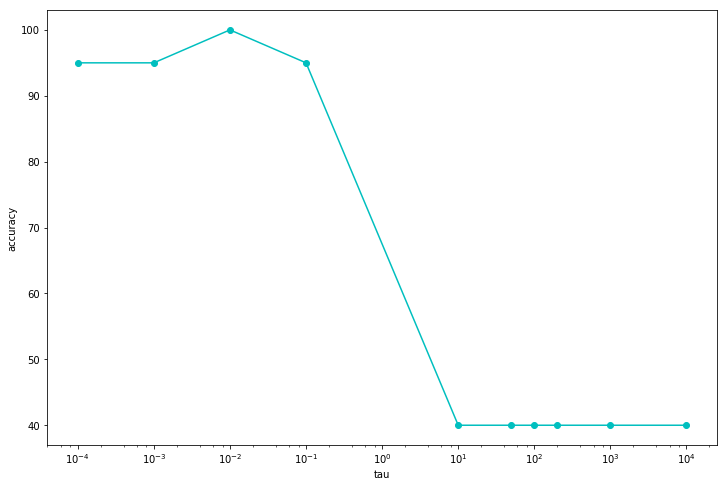
\includegraphics[width=\textwidth]{images/tau_versus_acc.png}
	\caption{Performance on the Iris dataset function of $\tau$}
	\label{fig:variation_tau}
\end{figure}

\subparagraph{Optional Part}
I randomly generated 2 clusters of data and I randomly picked tau in \texttt{[1e-3, 1e-2, 1e-1, 10, 100, 1e3]}. I plotted the data, the separating hyperplans found by our \texttt{barr\_method}
and the results we get using \texttt{LinearSVC} from \texttt{scikit-learn}. The results are displayed in Figure ~\ref{fig:random_test}

\begin{figure}[H] 
	\centering
	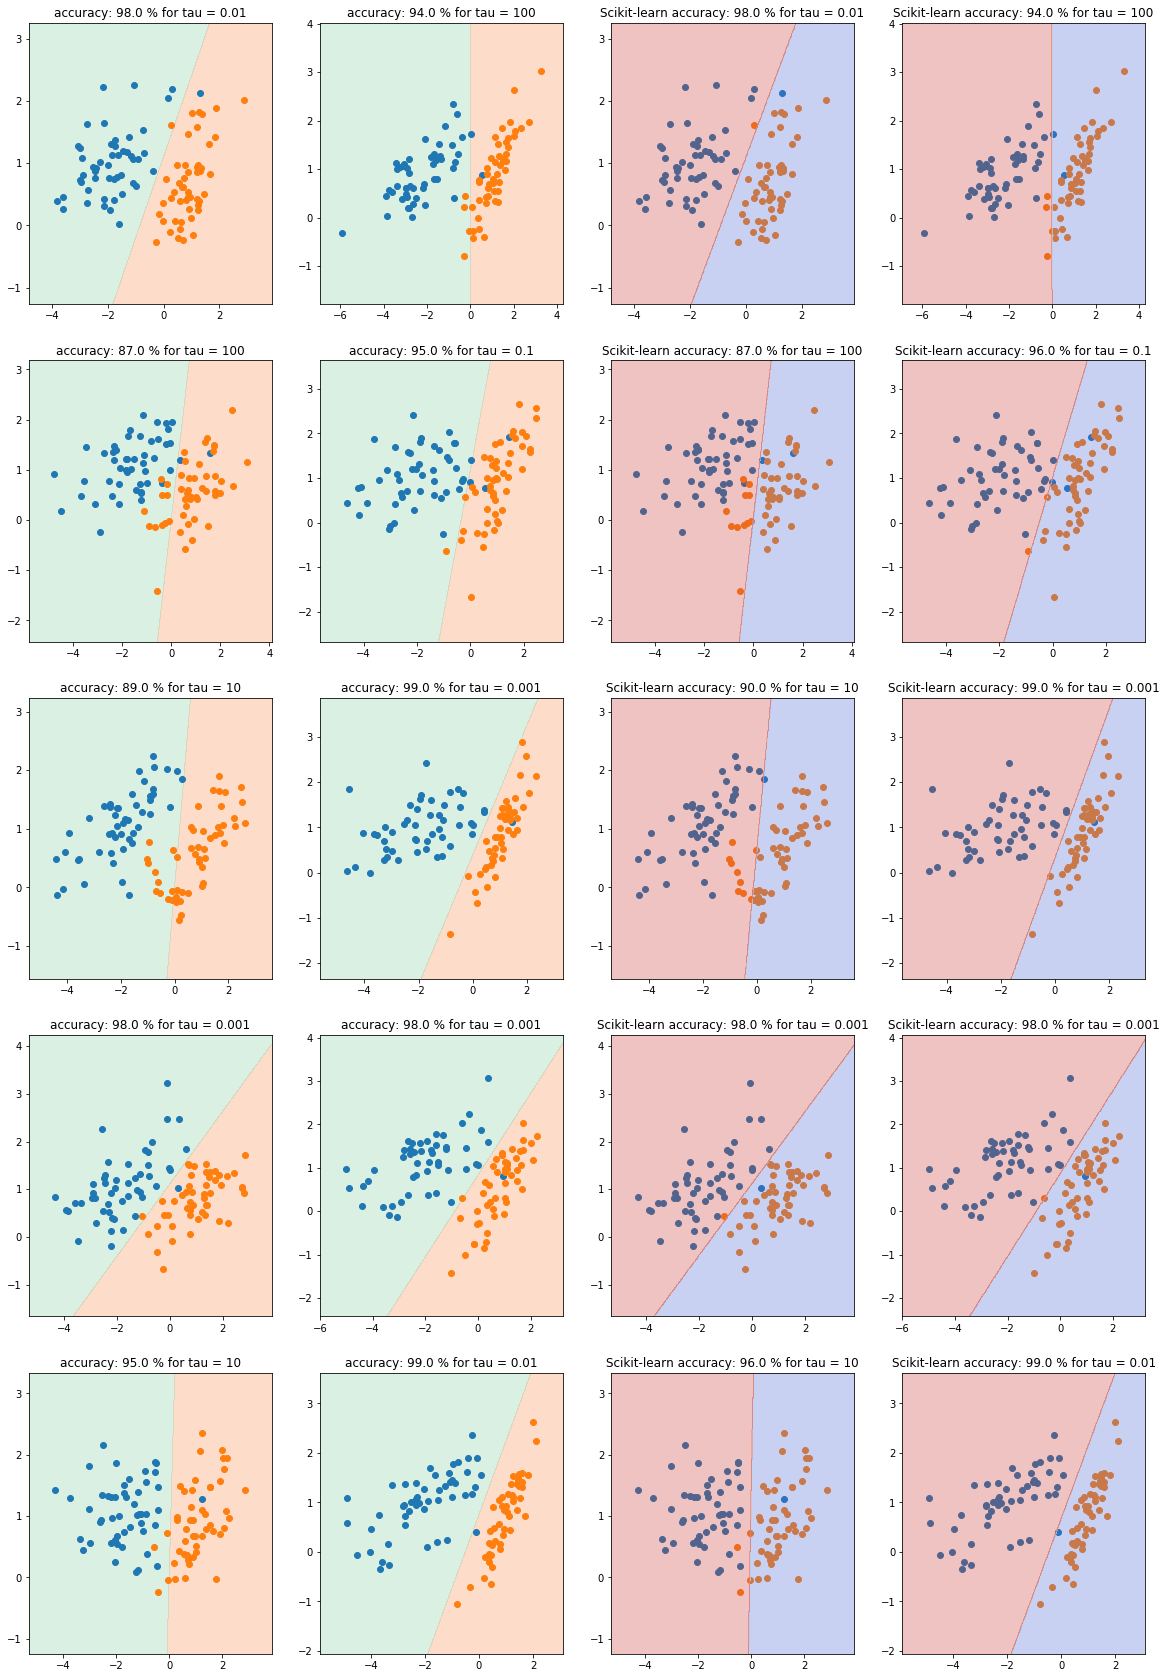
\includegraphics[width=\textwidth]{images/random_data.png}
	\caption{\textbf{Right}: Accuracies and hyperplans obtained using our implementation. \textbf{Left}: Accuracies and hyperplans obtained using \texttt{LinearSVC} from scikit-learn with the same parameters}
	\label{fig:random_test}
\end{figure}

We can see that the results between our implementation and scikit-learn is roughly the same. Yet, I don't understand the little variation between the two as I used the same
regularization parameter for both the \texttt{bar\_method} and the \texttt{LinearSVC} function. Moreover I've chosen the tolerance to be $10^{-9}$ for this question.

\paragraph{3.4 Duality gap versus Newton Iterations}
Here, the tolerance is: tol = 1e-6, $\tau=10$, $X$ is a matrix of features of Iris-versicolor and Iris-virginica only, and $y$ is a vector of classes (Iris-versicolor and Iris-virginica only).
Using the barrier method with both the damped Newton Method and the classic Newton Method (with backtracking line search) we can plot the duality gap versus Newton iterations for different
values of $\mu$ as shown in Figure~\ref{fig:duality_g}

\begin{figure}[H] 
	\centering
	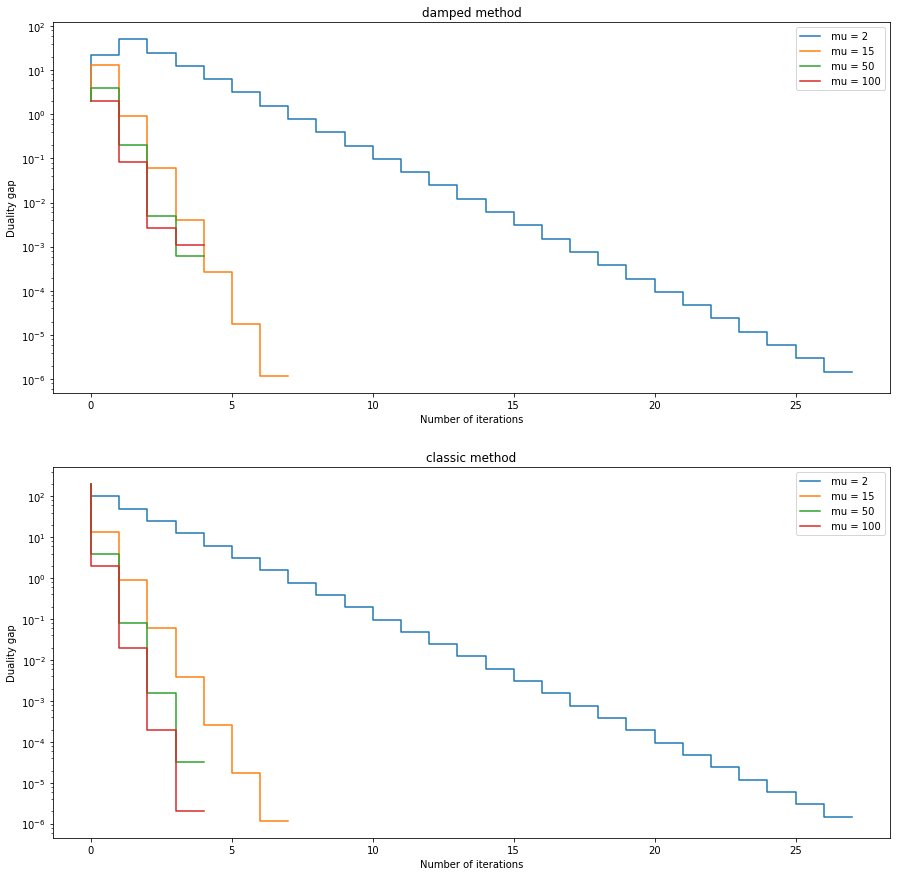
\includegraphics[width=\textwidth]{images/duality_gaps.png}
	\caption{\textbf{Up}: duality gaps using damped Newton Method, \textbf{Down}: duality gaps using Newton Method with line search}
	\label{fig:duality_g}
\end{figure}

We can see that the methods have more or less the same behavior. Yet, depending on the value of $\tau$ we can notice that the \textbf{Damped Newton method} takes usually more iterations to converge. So in a sense is not 'optimal'.

\end{document}
